\section{Hypothese}
Die Differenzierbarkeit von Farben beim Betrachten von Choroplethenkarten h�ngt vorallem von der Farbdistanz zwischen den Farben und der Anzahl der Farbklassen ab.

\section{Introduction}
From a designer's perspective, colors play an essential role in cartography. Nevertheless, according to \textcite{brychtova2017}, there is little research to empirically determine the minimum effective color distance to safely and correctly distinguish cartographic symbols. 

The ability to distinguish colors and shades of the same color plays an important role in cartography \parencite{coltekin2017}

Even subtle manipulation of color spacing shows significant effects on the impact on overall readability of a map (Brychtova et al. 2016; Brychtova and \i:iltekin 2015; Brychtova and \i:iltekin 2014; Brychtova 2014; Brychtova and Vondrakova
2014). 

Lack of proper visual distance in variables colour hue and colour value is a known contributor to legibility problems in map use tasks (Chesneau, 2007; Steinr�cken \& Pl�mer, 2013; Stigmar, 2010)\parencite{brychtova2015}

\subsection{Simple Choropleth maps}
Unlike chorochromatic maps, which visualize nominal (qualitative) data, simple choropleth maps have made it their business to display quantitative data in terms of area. In doing so, hue, saturation and brightness are used to show corresponding changes in the data. Although in theory choropleth maps are only useful for data related to areas (Bollmann et al. 2001), in practice they are also used for non-area related data. E.G. ? https://link.springer.com/content/pdf/10.1007/BF03545206.pdf

Some advantages of choropleth maps are e.g. the simplified visibility. For this, the data are classified. For example, one can distinguish between an equal interval and a quantile class division. With equal interval each class possesses the same size independently of its occupation, whereas with a quantile class division each class contains the same number of elements. Depending on the use case and data frequency, one or the other class division is more suitable, because they have a significant influence on the appearance of a map.
https://www.ssoar.info/ssoar/handle/document/67524

Due to the public availability of static data, the production of these maps is easy and can be linked, analyzed, classified and visualized with any suitable GIS software. https://link.springer.com/content/pdf/10.1007/BF03545206.pdf

\section{Basic color information}

\subsection{Human' color perception}
Although our current understanding is that color vision results from the response of three photoreceptor cells in the retina to incident light, their perception cannot be fully understood. This may be due to both individual and environmental factors that influence color perception. (Lafer-Sousa et al. 2015; Xiao et al. 2016) (Gegenfurtner and Sharpe 2001). .

Some of these factors can be, for example, the amount of light in the environment, shadows, surrounding materials, and reflectivity. In addition, the viewer's prior knowledge and cognitive biases play a significant role in color perception. (Derefeldt et al. 2004; Foster 2011). 

In addition, there is evidence that the number and distribution of photoreceptors in the eye influences what we see (Roy et al., 1991), and that our brain assumes a particular direction or light source e.g., Gegenfurtner et al. 2015; Lafer Sousa et al. 2015; Winkler et al. 2015. 

Thus, it can be said that the color perception of an individual is not stable over space and time. The same is true not only for individuals but also for groups.  

Nevertheless, there are many efforts to model and quantify color perception such as mathematical models that attempt to determine thresholds by which two colors or shades of the same color become distinguishable. 

This color distance describes a metric that quantifies the human ability to visually distinguish differences between two colors see chapter \ref{subsection:distance} \parencite{coltekin2017}.

\subsection{Color spaces}
There are a lot of color models that have set themselves the task of representing the logic of generating colors (Kuehni, 2001). These color models can be divided into four main groups: instrumental, pseudo-perceptual, colorimetric, and perceptual unitary color models.

Instrumental color models include, for example, RBG or CMYK. Pseudoperceptual color models are e.g. HVS or HSB, whereas colorimetric color models are represented e.g. by CIE 1931 XYZ. To the latter model (perceptually uniform) belong for example the Munsell system, CIELAB or CIELUV. The most frequently used color models are the CIE 1931 XYZ or CIELAB. 

A color space is understood to be all existing colors that can be represented e.g. by a screen, printer or the human eye, which are generated from a combination of the components of a model \parencite{munsell1915}.

\section{Criteria}

\subsection{Color distance}\label{subsection:distance}
Visual Distance in cartography is understood as a Measurement of Differences between visual variables such as size, shape, orientation and others \parencite{brychtova2015}. Here we focus on the variable of color hue and color value. The human perceived difference between two colors or color shades can be described as the color Distance. In other words, certain change of the colour in the perceptually uniform space produces equal change in human perception of that colour (Slocum et al. 2008 \parencite{brychtova2017}).

To describe the distance of two colors scientistis have developed a method to describe the color distance. To express color quantitatively a colour space corresponding to the human perception is needed. Such color spaces are called perceptually uniform or linear. The use of such color spaces try to ensure results of color distance which are proportional to the human perception (CIE, 2012 \parencite{brychtova2015}). Presently the CIEDE2000 model ($\Delta E_{00}$, equation defined in Sharma, Wu, \& Dalal, 2005 \parencite{brychtova2015}) is regarded as the best coinciding color space with visual perception. 
 
- RGB cause RGB represents how colors are created on most digital screens. 
- RGB values do not lead to a specific color if not related to an absolut color Space
- As a color space sRGB is selected, since sRGB color space is supported by most digital screens. Other color Spaces such as Adobe RGB are not fully suported by most digital screens. When puplishing a digital map creators should choose colors which can be displayed by most screens, therefore sRGB is the color space to choose.

\subsubsection{Equation}

- transforming sRGB Colors to CIE XYZ Colors. 
- Was ist CIE XYZ Colors
- For the transformation the sRGB values has to be in the range 0.0 - 1.0, therefore the most values have to be divided by 255 to nomalize them. 

\subsection{Number of classes}
\textcite{brychtova2017} makes the finding that with ColorBrewer 2.0 the color distance becomes smaller the more classes are used, which is to be expected. For the selected 18 sequential schemes, the color distance was analyzed and calculated between 3, 6 and 9 classes. These numbers of classes were selected according to \textcite{brychtova2017}, since they represent the minimum, maximum and middle of the class selection. Thus, the results (see table \ref{tab:classes}) show that the number of classes have an influence on how the distance of the colors is chosen and thus becomes distinguishable to the human eye. 

\begin{table}[h!]
\centering
\caption[Color distance depending on number of classes]{Color distance depending on number of classes \\ (According to \textcite{brychtova2017})}
	\begin{tabular}{c c c c }
		\hline
		\hline
		Number of classes & $\Delta E_{00}min$ & $\Delta E_{00}max$ & $\Delta E_{00}mean$ \\ 
		\hline
		\hline
		3 & 11.26 & 33.92 & 20.61 \\  
		6 & 6.24 & 26.44 & 12.41 \\
		9 & 3.04 & 20.46 & 10.28   
	\end{tabular}
\label{tab:classes}
\end{table}

\subsection{Further aspects}

\subsubsection{Spatial distance}
The greater the spatial distance between two color cells, the more the ability to distinguish the colors decreases. This is true for both sequential and qualitative schemes (Brychtova and \i:iltekin 2016). However, at a color distance of $\Delta E_{00}$ = 10, the accuracy of color discrimination increases, even at relatively large spatial distances. 

\subsubsection{Brightness of colors}

\section{Examples}
\subsection{ColorBrewer2.0}
Brewer and her colleagues (Brewer eta!. 2003; Brewer 1986, 1992, 1994, 1996, 1997, 1999; Harrower and Brewer 2003) did research on color, developing color schemes to viualize both quantitative and qualitative data. In the process, the online software ColorBrewer 2.0 was developed, which can be very helpful for many applications. ColorBrewer 2.0 offers the user a choice between 18 sequential, 9 divergent and 8 qualitative color schemes. Depending on the selection, a distinction can be made between 3 and 12 classes. They used Munsell diagrams to design color schemes that would maintain consistency in perceived color distances between classes \parencite{brychtova2017}. 

The Munsell Color System is a color system that is the first complete, most widely used, and still in use today. It is based on three essential criteria: Hue, Chroma and Value, with Hue being the most important criterion. Munsell chose five main hues: red (R), yellow (Y), green (G), blue (B) and purple (P). Now he subdivides the perceptible color nuances into further color tones, which are to represent the intermediate color tones: YR (yellow-red), GY (green-yellow), BG (blue-green), PB (purple-blue) and RP (red-purple). These ten hues are further subdivided a few times into ten gradations. Numbers from 0 to 10 are also added to the hues. Towards the outside, the saturation of the color (chroma) increases. The vertical center axis, which ranges from white (value 10) to black (value 0), which can be represented with colorants, is represented by the value. This results in a 10-row gray scale \parencite{munsell1915}.

\begin{figure}
	\centering
	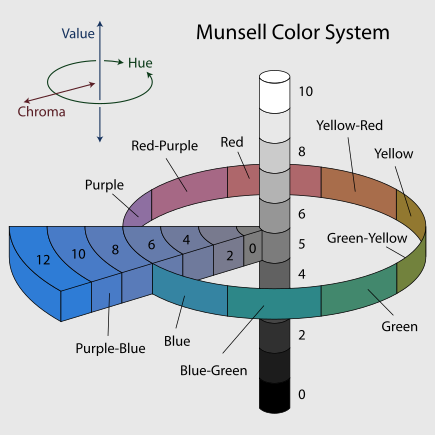
\includegraphics[width=0.6\linewidth]{source/images/munsell}
	\caption{Munsell Color System}
	\label{fig:munsell}
\end{figure}

\section{Conclusion}

%\bibliography